\documentclass[conference,compsoc]{IEEEtran}
\usepackage[T1]{fontenc}
\usepackage[utf8]{inputenc}
\usepackage{booktabs,tabularx,array,graphicx,amsmath,amssymb}
\usepackage{placeins}
\usepackage[dvipsnames,table]{xcolor}
\usepackage{tikz}
\usetikzlibrary{arrows.meta,positioning,fit}
\usepackage{pgfplots}
\usepgfplotslibrary{groupplots}
\pgfplotsset{compat=1.18}
\usepackage[hyphens]{url}
\usepackage{hyperref}
\hypersetup{hidelinks,pdfauthor={}}
% Avoid synthetic glyphs at math/text boundaries; preserve Unicode mappings.
\SetSymbolFont{letters}{normal}{OML}{lmm}{m}{it}
\SetSymbolFont{letters}{bold}{OML}{lmm}{b}{it}
\input{glyphtounicode}
\pdfgentounicode=1
\pdfglyphtounicode{space}{0020}
\ifdefined\pdfinterwordspaceoff\pdfinterwordspaceoff\fi
\newcolumntype{Y}{>{\raggedright\arraybackslash}X}
\newcolumntype{P}[1]{>{\raggedright\arraybackslash}p{#1}}
% Replace with the anonymized artifact URL before submission.
\newcommand{\artifacturl}{[anonymized artifact link]}
\newcommand{\papername}{Decoys That Do Work: Evaluating Executed Cover\\for LLM Agent Communication Privacy}
\title{\papername}
\author{}
\begin{document}
% Shared citation numbering for main paper and supplement.
\nocite{agentprint2025,jeong2026wra,dangol2026workflow,pouryousef2026traffic,song2026personafingerprint,kang2026whoseagent,fayolle2026webagents,shahriar2026agenttell,li2026ant,ayzenshteyn2025cheat,earlybird2025,whisperleak2025,timewilltell2024,wu2026cacheprune,juarez2014critical,mathews2023critical,wang2017walkietalkie,gong2020front,tramer2020adaptive,weiss2024prompt,carlini2024timing,ahmed2023voice,mcp2025transports,rfc9113,rfc8446,uitraces2026,roh2026spillage,chen2010web,chapman2011blackbox,reynolds2006wap5,tak2009vpath,dyer2012peekaboo,trimananda2020pingpong,apthorpe2019stp}

\nocite{duan2026privacytrace,yao2026intentminer}
\nocite{sirinam2018df,bhat2019varcnn,rfc9114,rfc9000}
\nocite{song2026redefining,zavrak2026content}

\nocite{guan2021bapm,deng2023ares,wang2016realistic,hayes2016kfp}

\nocite{zhao2026agenttrace,ediga2026trace,borysenko2026http,borysenko2026short,reworr2024honeypot}

\nocite{arp2022dos}

\nocite{yao2024survey,shahriar2025survey,ferrag2025survey}
\nocite{langchain2025langgraph}

\nocite{debenedetti2025camel,costa2025fides,shi2025progent,yao2024taubench,debenedetti2024agentdojo}
\nocite{cai2014tamaraw}

\raggedbottom
\pagestyle{plain}
\maketitle
\thispagestyle{plain}
\begin{abstract}
When an adversary observes the last hop to a third-party tool, or is the tool, an LLM Agent's privacy cover cannot be discarded before it reaches the service: decoys must execute as real calls, consuming quota, touching state and possibly re-entering the planner's context. We characterize when cover must execute, classify executed cover by termination, state, feedback and dispatcher, and propose an evaluation that binds residual inference, task completion, business-state integrity and cost to the same protected executions. In 3,000 single-host executions with two fixed-weight planners over MCP and TLS~1.3/HTTP/2, controller cover that skips the model wait is removable: given call boundaries, label-free timing removal raises recognition from 75 to 112 (Qwen) and from 80 to 108 (Llama) of 120 tasks. History-matched dispatch removes this shortcut, yet adapted attacks still recognize 93--106/120, a significant gain in three of four cells; without call boundaries, the prespecified removal attack loses its advantage. Against a shadow planner, the strongest tested attack reaches but does not exceed a pair-ambiguity floor we derive (7/12 for one shadow), which only more shadows or label-aware sampling can lower. In a stress control, goal completion misses collateral state damage in 95 of 102 completed tasks. Existing Agent defenses report an adapted attacker and matched task utility in no common setting; applying our protocol with declared tolerances shows that the policy to deploy depends on the declared observer.
\end{abstract}

\section{Introduction}\label{sec:intro}
An LLM Agent receives a support ticket, checks an order and submits a refund through a third-party commerce service. The traffic is encrypted, yet an observer of the path to that service sees which endpoints are contacted, how large each exchange is and how long the Agent waits between them. Recent work shows that such metadata reveal prompts, tasks, workflows and user traits~\cite{jeong2026wra,dangol2026workflow,pouryousef2026traffic,li2026ant}.

A defender who wants to hide the refund can add decoy calls. Classical traffic-analysis defenses discard their cover at a cooperating endpoint before it reaches an application~\cite{apthorpe2019stp}. The commerce service is not under the defender's control and offers no such endpoint. A relay could move the discard point, but the hop from the relay to the service remains visible to whoever watches it, and the service itself sees every request it receives. Against these observers, decoys must arrive as real requests and \emph{execute}. Executed cover then has two outputs: a communication trace and application work, which can consume quota, touch other objects and re-enter the planner's context.

This paper asks how such cover should be designed and evaluated. Existing Agent studies do not answer it. In the four query/workflow privacy settings we could locate, none reports both an attack adapted to the protected traffic and original-task utility under the same intervention~\cite{jeong2026wra,dangol2026workflow}. Website-fingerprinting research already requires adapted attacks and matched costs~\cite{juarez2014critical,mathews2023critical}; Agent execution adds business state and the process that generates cover.

\begin{figure*}[t]
\centering
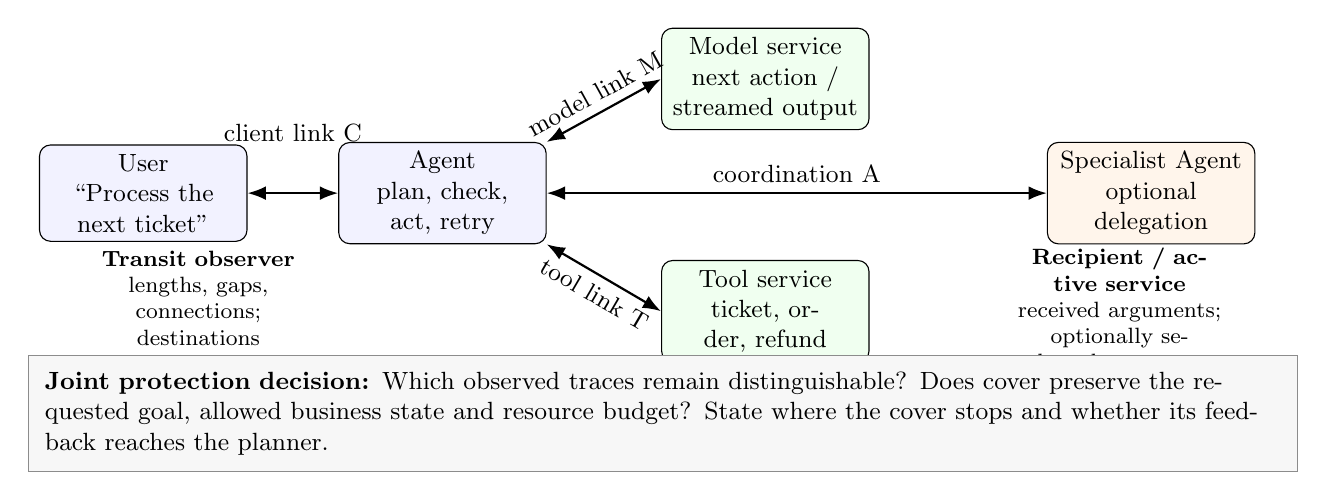
\begin{tikzpicture}[x=1cm,y=1cm,font=\small,>=Latex]
\tikzset{box/.style={draw,rounded corners,align=center,minimum height=.85cm,text width=2.4cm},
 note/.style={align=center,font=\footnotesize,text width=3.1cm}}
\node[box,fill=blue!5] (u) at (1.3,1.15) {User\\``Process the next ticket''};
\node[box,fill=blue!5] (a) at (5.1,1.15) {Agent\\plan, check, act, retry};
\node[box,fill=green!6] (m) at (9.2,2.6) {Model service\\next action / streamed output};
\node[box,fill=green!6] (t) at (9.2,-.35) {Tool service\\ticket, order, refund};
\node[box,fill=orange!8] (d) at (14.1,1.15) {Specialist Agent\\optional delegation};
\draw[<->,thick] (u)--node[above,yshift=15pt]{client link C}(a);
\draw[<->,thick] (a.north east)--node[above,sloped]{model link M}(m.west);
\draw[<->,thick] (a.south east)--node[below,sloped]{tool link T}(t.west);
\draw[<->,thick] (a.east)--node[above]{coordination A}(d.west);
\node[note] at (2.0,-.35) {\textbf{Transit observer}\\lengths, gaps, connections;\\destinations when available};
\node[note] at (13.7,-.35) {\textbf{Recipient / active service}\\received arguments;\\optionally selected responses};
\node[draw=black!45,fill=black!3,align=left,text width=15.7cm,inner sep=6pt] at (7.9,-1.65) {
\textbf{Joint protection decision:} Which observed traces remain distinguishable? Does cover preserve the requested goal, allowed business state and resource budget? State where the cover stops and whether its feedback reaches the planner.};
\end{tikzpicture}
\caption{Running support-ticket example and observation rights. A tool result returns to the Agent and can enter the next model request. Each encrypted link exposes its own traffic shape; a recipient additionally sees the request addressed to it. Concurrent tickets may share a connection on either link. The arrows represent application communication, not a one-to-one mapping from tool events to packets.}
\label{fig:chain}
\end{figure*}


\paragraph{Approach}
We characterize when cover must execute, classify executed cover along four axes (termination, state, feedback and dispatcher), and define an evaluation that binds residual inference, requested-goal completion, business-state integrity and resource cost to the same protected executions. We apply it to 3,000 live executions of two fixed-weight planners, Qwen3:8B and Llama3.1:8B, over MCP and TLS~1.3/HTTP/2 on one host, comparing four cover dispatchers against no cover.

\paragraph{Findings}
\begin{itemize}
\item \textbf{The dispatcher leaks.} Honest calls follow a model decision. Controller cover that skips that wait is removable: given call boundaries, label-free gap removal raises recognition from 75 to 112 (Qwen) and from 80 to 108 (Llama) of 120 tasks.
\item \textbf{History matching hides the shortcut, not the signal.} Sampling honest gaps defeats the simple removal, yet adapted attacks still recognize 93--106/120, a significant gain in three of four model/arm cells. Without call boundaries, the prespecified removal attack loses its advantage.
\item \textbf{Planner shadows have a computable floor.} A second planner on an independent ticket leaves an idealized attacker the modal-label guess among the chains. We derive this pair-ambiguity floor $P^*(k)$ for $k$ shadows; with one shadow it is 7/12, and the strongest tested attack reaches but does not exceed it, at about twice the model tokens.
\item \textbf{Goal completion is not state integrity.} In a stress control where cover writes to live state, 95 of 102 completed Qwen tasks leave collateral damage that a goal check misses.
\item \textbf{The decision depends on the observer.} Under illustrative tolerances, only the shadow passes against a call-window observer, whereas the cheaper history-concurrent policy passes for Qwen when call boundaries are withheld.
\end{itemize}

\paragraph{Contributions}
(1) A threat model and necessity rule for executed cover, and a four-axis design space (Sections~\ref{sec:threat}--\ref{sec:design}). (2) A joint evaluation protocol with a derived pair-ambiguity floor for planner cover (Section~\ref{sec:method}). (3) A live measurement of dispatch leakage, boundary-free recognition, shadow floors and business-state effects, with per-policy decisions (Sections~\ref{sec:setup}--\ref{sec:results}). Appendix~\ref{app:map} maps all forty-four existing Agent side-channel settings that motivate the protocol.

\section{Background and Motivation}\label{sec:background}

\subsection{Agent communication}
An Agent uses an LLM to choose actions, and external feedback can change its later actions or termination. Figure~\ref{fig:chain} shows the links of the running example: client--Agent, Agent--model, Agent--tool and inter-agent coordination. A tool result returns to the Agent and can enter the next model request. Tools are commonly reached through the Model Context Protocol (MCP), either over local stdio or over Streamable HTTP~\cite{mcp2025transports}. Remote connections typically use TLS~1.3 and HTTP/2, which encrypt content but expose record lengths, directions and timing, and multiplex several request streams on one connection~\cite{rfc8446,rfc9113}. A captured packet, TLS record, HTTP stream, tool call and complete task are therefore different units, and a boundary supplied by an evaluator is prior information, not an attacker output.

\subsection{Communication side channels in Agents}
A small but growing literature shows that Agent traffic leaks. Transit observers recover research prompts and user traits from contacted domains and timing~\cite{jeong2026wra}, workflow classes from inter-agent communication graphs~\cite{dangol2026workflow}, and tasks or misuse from model-link and egress traffic~\cite{pouryousef2026traffic,li2026ant,agentprint2025}. Contacted recipients fingerprint Agent clients and models from protocol headers, terminal commands and tool-call arguments~\cite{kang2026whoseagent,fayolle2026webagents,ediga2026trace,zhao2026agenttrace,duan2026privacytrace}, and active defenders plant lures for Agent adversaries~\cite{ayzenshteyn2025cheat,reworr2024honeypot}. Appendix~\ref{app:map} maps all forty-four settings from fifteen such studies by observer access, target, unit and intervention. Most evaluate recognition; few evaluate a protection.

\subsection{How traffic defenses are evaluated}
Website-fingerprinting (WF) work has established what a defense evaluation must contain: realistic observer information and splits, attacks adapted to the protected distribution, and overheads measured on the same traffic~\cite{juarez2014critical,mathews2023critical,dyer2012peekaboo}. Adaptive-attack and ML-security guidance make the same demands~\cite{tramer2020adaptive,arp2022dos}. Classical defenses pad, pace or add dummy traffic, and their cover never reaches an application~\cite{wang2017walkietalkie,gong2020front,juarez2016wtfpad,apthorpe2019stp}. State-aware Agent benchmarks check environment outcomes~\cite{yao2024taubench,debenedetti2024agentdojo} but do not measure traffic.

\subsection{The gap}\label{sec:gap}
Table~\ref{tab:availability} applies those requirements to the four Agent query/workflow privacy settings we located. WRA's five research decoys lower query recovery from .770 to .565, but its report-utility scores of 8.55 and 8.54 belong to a different intervention that changes destination visibility~\cite{jeong2026wra}. The communication-graph study refits its attacker on live OHTTP captures and reports about thirteen-fold bytes, but no original-task outcome under that intervention~\cite{dangol2026workflow}. No setting reports both an adapted attacker and matched utility, and the only executed-cover setting reports no matched utility at all. This is a statement about four settings from two sources, not a field-wide frequency; it shows that the measurements a deployment decision needs have not yet been made together.

\begin{table*}[t]\centering\small
\caption{Evidence located in the retained records. Counts use eligible settings; the second column also gives distinct sources. ``Not located'' leaves evidence unresolved within the inspected scope. These counts describe availability, not study quality or checklist validity.}\label{tab:availability}
\setlength{\tabcolsep}{4pt}
\begin{tabularx}{\textwidth}{@{}P{.28\textwidth}P{.15\textwidth}P{.11\textwidth}Y@{}}\toprule
Question & Eligible settings / sources & Located & Supporting settings and consequence \\\midrule
Protected-condition attack adaptation & 4 / 2 & 2/4 & Communication graphs: transformed captures and live OHTTP. Both come from one preprint. \\\addlinespace[3pt]
Original-task utility under the same intervention & 4 / 2 & 1/4 & WRA visibility comparison. It does not price WRA's executed-decoy condition. \\\addlinespace[3pt]
Adaptation and original-task utility in one setting & 4 / 2 & 0/4 & Adaptation and utility are located in different records; transport cost alone does not fill the task-outcome field. \\\addlinespace[3pt]
Original-task utility for executed cover & 1 / 1 & 0/1 & WRA's five research decoys report recovery and extra research; matched original-task utility is not located. \\\bottomrule
\end{tabularx}
\end{table*}


\section{Threat Model}\label{sec:threat}
\paragraph{Assets and adversary}
The private target is the user's requested task, here one of six support actions. The defender controls the Agent and its controller, and may run relays, but does not control third-party tool services. We consider three observers, distinguished by their rights. A \emph{transit observer} sees connection destinations, directions, ciphertext lengths and times on the links it watches. A \emph{recipient} additionally reads the requests addressed to it, including arguments. An \emph{active auditor} also chooses probes. Identifying a requested action does not establish whether it was authorized; that needs the principal and policy context. Table~\ref{tab:deployment-access} maps these rights to common deployments and to the existing evidence for each view.

\begin{table*}[t]\centering\small
\caption{Deployment and access map. The configurations are analyst-defined; cited settings test the listed view, not every component of the deployment. A gateway's plaintext access requires TLS termination.}\label{tab:deployment-access}
\setlength{\tabcolsep}{4pt}
\begin{tabularx}{\textwidth}{@{}P{.18\textwidth}P{.25\textwidth}P{.28\textwidth}Y@{}}\toprule
Deployment & Observer and permitted view & Existing evidence for that view & Protection consequence \\\midrule
Enterprise egress & A transit monitor sees routed model/tool flows, sizes, times and any exposed destination association. & WRA: supplied research-domain traces; ANT and cloud benchmark: model/combined traffic~\cite{jeong2026wra,li2026ant,pouryousef2026traffic}. & Specify which services cross the monitored egress. A union of flows is available only when the monitor can observe them. \\\addlinespace[3pt]
Shared gateway or relay & Transit sees multiplexed gateway output. A terminating gateway can additionally read addressed requests. & Live OHTTP: passive-link inference under stated relay trust~\cite{dangol2026workflow}; PrivacyTrace: semantic recipient/gateway access~\cite{duan2026privacytrace}. & Separate relay association protection from content trust. Connection sharing changes the observation unit. \\\addlinespace[3pt]
Local model, remote tools & An external observer sees remote tool traffic; the local model call has no corresponding external network leg. & WRA's destination-recovery mechanism is relevant to tool egress~\cite{jeong2026wra}; whole-deployment protection is untested in the mapped comparison. & Evaluate tool and downstream calls. Do not import a remote-model attack score into an absent network leg. \\\addlinespace[3pt]
Cloud model, remote tools & An authorized vantage may see either or both encrypted legs. A contacted tool sees its own arguments. & ANT/cloud benchmark test model traffic~\cite{li2026ant,pouryousef2026traffic}; PrivacyTrace tests recipient-visible representations~\cite{duan2026privacytrace}. & Check permitted model and tool views after the intervention; recipients and passive monitors need different protections. \\\bottomrule
\end{tabularx}
\end{table*}


\paragraph{When cover must execute}
Transport cover ends before a business tool, at an endpoint the defender controls~\cite{apthorpe2019stp}. That endpoint must sit after the observer, or the observer sees it discard the cover. A defender can move the endpoint, for example to a relay outside a monitored egress, but the segment from the last defender-controlled hop to a third-party service remains. If the adversary observes that segment, or is the service, every request it sees must be real (Table~\ref{tab:cover-necessity}). Executed cover then follows from the deployment rather than from a design preference.

\begin{table}[t]\centering\footnotesize
\caption{When cover must execute. Transport cover needs a defender-controlled terminator after the observer and before the business service. A relay can move the terminator but not past the final hop to a third-party service; an observer of that hop, or the service itself, sees only real calls.}\label{tab:cover-necessity}
\setlength{\tabcolsep}{3pt}
\begin{tabularx}{\columnwidth}{@{}P{.27\columnwidth}P{.2\columnwidth}Y@{}}\toprule
Observer $\to$ service & Terminator after observer? & Cover that can work \\\midrule
Egress $\to$ own service & Yes (own tunnel) & Transport cover suffices~\cite{apthorpe2019stp} \\\addlinespace[2pt]
Egress $\to$ third-party SaaS or remote MCP & Only via a relay outside the egress & Transport cover against the egress alone; executed cover if the relay's upstream hop is observed \\\addlinespace[2pt]
Recipient (tool provider) & No & Executed cover whose arguments must also be plausible to the recipient \\\addlinespace[2pt]
TLS-terminating gateway & After gateway only & Executed cover, or trust the gateway with content \\\bottomrule
\end{tabularx}\end{table}


\paragraph{Observer in this paper}
Our measurements use a transit observer on the final hop to seven tool services that stand for third-party tools, with no defender relay in between. It receives destinations, ciphertext bytes and TLS record completion times. Section~\ref{sec:dispatch} additionally supplies episode and call windows, an evaluator privilege that Section~\ref{sec:noboundary} withdraws. The recipient view, where decoy arguments are also visible, is part of the threat model but not of these measurements (Section~\ref{sec:limits}). The adversary may train on traffic generated under the same cover policy; the attack suite therefore includes classifiers and cover-removal models fitted on protected training executions, alongside attacks frozen on unprotected traffic.

\section{The Executed-Cover Design Space}\label{sec:design}
\paragraph{Four axes}
We classify a cover policy along four axes (Table~\ref{tab:cover-taxonomy}). \emph{Termination} and \emph{state} determine what business work cover performs: a disposable copy, read-only access, an isolated clone or production state. \emph{Feedback visibility} determines whether cover responses enter later model requests and can change the real planner's decisions. The \emph{dispatcher}, the process that decides when cover is sent, determines whether cover inherits the timing of honest calls. Honest calls follow a model decision; a controller that inserts cover without waiting for the model creates a timing signature that the first three axes do not capture. Our live study varies the dispatcher while holding termination (an isolated clone) and feedback (hidden) fixed; an earlier state control varies termination and feedback.

\begin{table*}[t]\centering\small
\caption{Cover taxonomy. Each policy is classified by where it terminates and what state it touches, whether its responses reach the real planner, and which process dispatches it. The last column names the evaluation in which the policy is measured; S1 is the earlier state control and Section~\ref{sec:dispatch} the live timing study.}\label{tab:cover-taxonomy}
\setlength{\tabcolsep}{4pt}
\begin{tabularx}{\textwidth}{@{}P{.17\textwidth}P{.26\textwidth}P{.13\textwidth}P{.2\textwidth}Y@{}}\toprule
Policy & Terminates at / state touched & Feedback to planner & Dispatcher & Measured in \\\midrule
Transport cover & Tunnel endpoint before the service; no business state & No & Sender schedule & STP~\cite{apthorpe2019stp}; WF padding~\cite{juarez2016wtfpad,gong2020front} \\
Proxy discard & Defender proxy computes on a disposable copy & No & Controller & S1 \\
Read cover & Real service; reads only & No & Controller & S1 \\
Isolated execution & Real service on a persistent clone & No / yes & Controller & S1 (hidden and visible); all live cover arms \\
Live write & Real service on production state & No & Controller & S1 (stress control) \\
Research decoys & Real third-party Web destinations & Not located & Decoy generator & WRA~\cite{jeong2026wra} \\\midrule
Immediate & Isolated clone & No & Controller, directly after an honest response & Section~\ref{sec:dispatch} (calibration) \\
History-matched & Isolated clone & No & Controller, training-gap and duration samples; sequential or concurrent & Section~\ref{sec:dispatch} \\
Planner shadow & Isolated clone; separate planner context & No & Second planner on an independent ticket & Section~\ref{sec:dispatch} \\\bottomrule
\end{tabularx}\end{table*}


\paragraph{The execution contract}
Because executed cover performs work, a policy must satisfy a contract as well as a privacy target. The contract names the objects and transitions cover may touch, the quota, token and latency budgets it may consume, and the feedback it may expose to the real planner. Isolation prevents direct writes to production state but still consumes compute and can change scheduling; a response hidden from the planner does not undo the operation that produced it. A requested goal can complete while another order, a shared quota or a ledger is wrong, so the contract separates three outcomes: requested-goal completion, violations of declared business invariants, and resource use. For a synthetic fixture whose intended transition is fully specified, exact state equality is the invariant; in production, invariants must admit legitimate concurrent updates.

\paragraph{Where executed cover sits among defenses}
Name hiding and relays change destination association; padding changes lengths; pacing changes timing~\cite{wang2017walkietalkie,gong2020front,juarez2016wtfpad}. These layers remain useful, and Table~\ref{tab:cover-necessity} shows when transport cover suffices. Executed cover is the remaining option when the observed hop ends at a service the defender does not control. Model services add their own signals, such as token streams, cache behavior and token counts~\cite{weiss2024prompt,whisperleak2025,earlybird2025,timewilltell2024,carlini2024timing}; a tool-side cover policy does not shape later model requests. Appendix~\ref{app:defense} summarizes what each defense layer requires the defender to control, the costs to measure together and the exposure that remains.

\section{Evaluation Methodology}\label{sec:method}
\subsection{Joint evaluation protocol}
Privacy, task success, business state and cost must refer to the same intervention and evaluation population. The protocol has four steps; Table~\ref{tab:joint-checklist} is its reporting form.
\begin{enumerate}
\item \textbf{Specify observations and execution authority.} Name the hidden target, the visible links, recipient rights and any supplied boundaries. State where cover ends, which state it can access and whether its responses reach the planner.
\item \textbf{Specify the contract and tolerances.} Define the requested goal, allowed collateral transitions, and the inference, quota, token and latency tolerances, before measuring.
\item \textbf{Measure matched executions and adapted attacks.} Pair baseline and policy on the same workload. Include cover-removal and schedule-aware attacks, report the strongest tested residual inference, and take task, state and cost outcomes from those protected runs.
\item \textbf{Decide.} A policy fails if any declared tolerance is exceeded: an execution outside its state or resource contract fails even when its goal passes. Passing a finite attack suite is not a secrecy proof.
\end{enumerate}

\begin{table}[t]\centering\footnotesize
\caption{Joint evaluation checklist for one intervention and population. Attach evidence or state the missing item; goal completion and whole-state correctness are separate fields.}\label{tab:joint-checklist}
\begin{tabularx}{\columnwidth}{@{}lY@{}}\toprule
$\square$ & Hidden target, population, prior or base rate \\
$\square$ & Allowed observations and supplied boundaries \\
$\square$ & Cover termination, privileges and isolation \\
$\square$ & Planner-visible cover feedback and dispatcher \\
$\square$ & Declared tolerances: inference, goal, state, tokens, bytes, latency \\
$\square$ & Adapted attacks and largest tested residual \\
$\square$ & Original-task attempts, completion and failures \\
$\square$ & Business invariants and violations \\
$\square$ & Matched bytes, latency, tokens and quota \\\bottomrule
\end{tabularx}\end{table}


\subsection{Attacks and statistics}\label{sec:stats}
Each condition has its own attack suite, fitted on its training split. Size-only attacks are logistic regression (LR) and a 300-tree random forest (RF) on destinations and ciphertext sizes, a classifier frozen on no-cover traffic, and last- and penultimate-destination rules. Timing attacks add timing features, supervised and label-free gap removal, context-aware removal and joint decoding; Supplement S2.3 defines them. The following conventions apply to every result. \emph{Sel.}\ is the attack chosen on validation data before test scoring, and primary tests use only these choices. \emph{Max} is the largest test count in a finite suite; it is descriptive and is not an upper bound on inference. \emph{Exploratory} marks an analysis designed after test results were seen. Paired tests are exact McNemar tests with Holm correction within each prespecified family; intervals use 10,000 action-stratified fixture bootstraps and condition on the fitted attacks and designed workload.

\subsection{A floor for planner cover}\label{sec:floor}
Planner cover runs $k$ complete shadow executions beside the real one. Consider an idealized attacker who separates all $k+1$ chains perfectly and recovers each chain's label, but cannot tell which chain is real. If the real chain is exchangeable with the shadows, then given the multiset of labels the real label is $c$ with probability $n_c/(k+1)$, where $n_c$ counts the chains labeled $c$. The best guess is a modal label, which succeeds with probability
\[P^*(k)=\frac{\mathbb{E}[\max_c n_c]}{k+1}.\]
With one shadow and six uniform classes, $P^*(1)=\tfrac16+\tfrac56\cdot\tfrac12=\tfrac7{12}$. Table~\ref{tab:shadow-floor} gives exact values. Drawing shadow labels without replacement from the classes other than the real one makes all labels distinct and gives $1/(k+1)$, while keeping each shadow's marginal label uniform. $P^*(k)$ is a reference, not a bound: an attacker who learns which chain is real exceeds it, and reused real fixtures with their own cache histories make exchangeability an idealization. The right comparison for a shadow policy is therefore $P^*(k)$, not the uniform $1/6$.

\begin{table}[t]\centering\footnotesize
\caption{Pair-ambiguity floor $P^*(k)$ for $k$ shadow planners and six classes, computed exactly (\texttt{experiment/shadow\_floor.py}). \emph{iid}: shadow labels drawn uniformly; \emph{distinct}: drawn without replacement from classes other than the real one. Tokens are nominal planner multiples. Only $k=1$, iid, was run.}\label{tab:shadow-floor}
\setlength{\tabcolsep}{4pt}
\begin{tabular}{@{}rrrrl@{}}\toprule
$k$ & iid & distinct & Tokens$\times$ & Live result ($k=1$) \\\midrule
0 & 1.000 & -- & 1 & \\
1 & .583 & .500 & 2 & Max 70 / 64 of 120 \\
2 & .491 & .333 & 3 & \\
3 & .456 & .250 & 4 & \\
4 & .428 & .200 & 5 & \\\midrule
\multicolumn{5}{@{}l}{Realized $k=1$ floor on the test split: 70.5/120 (21 matching labels)} \\\bottomrule
\end{tabular}\end{table}


\section{Experimental Setup}\label{sec:setup}
\paragraph{Workload and planners}
Each fixture is a synthetic support ticket requesting one of six business actions over a state with three orders, a customer address, a compensation quota, an escalation status and a ledger. LangGraph~\cite{langchain2025langgraph} alternates model decisions with real tool calls to seven MCP Streamable HTTP services over TLS~1.3/HTTP/2, with request and response bodies padded to 4,096 and 16,384 bytes. Two fixed-weight planners, Qwen3:8B and Llama3.1:8B, run at temperature zero with weights pinned by layer hashes. Each planner executes 300 fixtures per condition: 120 training, 60 validation and 120 paired test fixtures, balanced over the six actions. The label is the requested action, and wrong or failed executions remain in every denominator.

\paragraph{Cover policies}
All four cover arms execute cover on an isolated clone and hide its responses from the real planner; they differ only in the dispatcher (Figure~\ref{fig:dispatch}). \emph{Immediate} cover follows an honest response directly. \emph{History} cover samples a training-only honest gap and service duration, waits in real time and holds the response for the sampled minimum; the \emph{sequential} variant blocks the real chain and the \emph{concurrent} variant overlaps real model inference. \emph{Shadow} runs a complete second planner on an independent ticket whose action is drawn uniformly, and a fair draw decides which chain starts first. Calls to the same service serialize. The five conditions give 3,000 main episodes and 600 shadow chains.

\begin{figure}[t]\centering
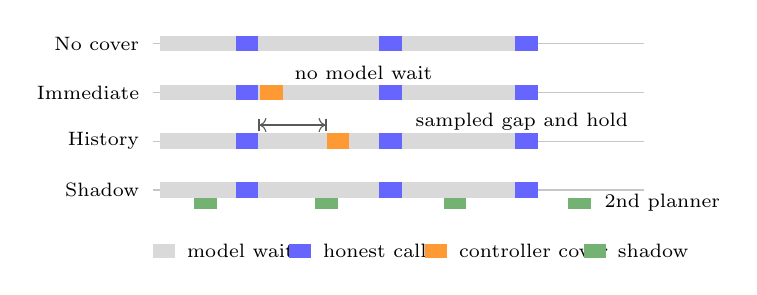
\begin{tikzpicture}[x=.48cm,y=.62cm,font=\scriptsize]
\def\bar#1#2#3#4{\fill[#4] (#1,#3-.16) rectangle (#2,#3+.16);}
\foreach \y/\n in {4/No cover,3/Immediate,2/History,1/Shadow}{
 \node[anchor=east] at (-.1,\y) {\n};
 \draw[gray!45] (0,\y)--(13,\y);
 \bar{0.2}{2.2}{\y}{gray!30}\bar{2.2}{2.8}{\y}{blue!60}
 \bar{2.8}{6.0}{\y}{gray!30}\bar{6.0}{6.6}{\y}{blue!60}
 \bar{6.6}{9.6}{\y}{gray!30}\bar{9.6}{10.2}{\y}{blue!60}}
% immediate cover: right after the honest response
\bar{2.85}{3.45}{3}{orange!80}
\node[anchor=west] at (3.5,3.4) {no model wait};
% history cover: after a sampled gap
\bar{4.6}{5.2}{2}{orange!80}
\draw[|<->|,gray!70!black] (2.8,2.33)--(4.6,2.33);
\node[anchor=west] at (6.7,2.4) {sampled gap and hold};
% shadow chain: its own model waits
\foreach \a in {1.1,4.3,7.7,11.0}{\fill[green!45!black!55] (\a,.62) rectangle (\a+.6,.84);}
\node[anchor=west] at (11.7,.73) {2nd planner};
% legend
\begin{scope}[yshift=-.25cm]
\fill[gray!30] (0,0) rectangle (.6,.3); \node[anchor=west] at (.65,.15) {model wait};
\fill[blue!60] (3.6,0) rectangle (4.2,.3); \node[anchor=west] at (4.25,.15) {honest call};
\fill[orange!80] (7.2,0) rectangle (7.8,.3); \node[anchor=west] at (7.85,.15) {controller cover};
\fill[green!45!black!55] (11.4,0) rectangle (12.0,.3); \node[anchor=west] at (12.05,.15) {shadow};
\end{scope}
\end{tikzpicture}
\caption{Dispatchers in the live study. Honest calls follow a model wait. Immediate cover follows the previous response without one, which label-free gap removal exploits. History-matched cover samples a training gap and response hold. Shadow calls come from a second planner, so their gaps are model waits too.}\label{fig:dispatch}
\end{figure}

\begin{table}[t]\centering\footnotesize
\caption{Study map. Each population answers one question and keeps its own denominators and statistical role.}\label{tab:study-map}
\setlength{\tabcolsep}{3pt}
\begin{tabularx}{\columnwidth}{@{}P{.2\columnwidth}P{.25\columnwidth}Y@{}}\toprule
Study & Population; observer & Question; role \\\midrule
Live timing (\S\ref{sec:dispatch}) & 3,000 episodes + 600 shadow chains; call windows, TLS record times & Does the dispatcher expose cover? Primary families P, R, C \\\addlinespace[2pt]
Record-only (\S\ref{sec:noboundary}) & Same episodes; no call boundaries & How much survives without supplied boundaries? Retrospective; one primary pair \\\addlinespace[2pt]
State control (\S\ref{sec:state}; S1) & 3,600 episodes; call windows, sizes only & Does goal completion miss collateral state? Primary state family \\\addlinespace[2pt]
Forwarding pilot (S10) & 3,120 local + 192 hosted & Feedback attribution; inconclusive, supplement only \\\bottomrule
\end{tabularx}\end{table}


\paragraph{Studies}
Table~\ref{tab:study-map} lists the populations. The live timing study and its record-only reanalysis answer the privacy questions. A separate earlier state control on the same workload varies termination and feedback across six policies, including a deliberately harmful live-write arm, to test whether goal completion misses collateral state. A forwarding pilot appears only in Supplement S10. All runs use one host over loopback with synthetic tools; Section~\ref{sec:limits} states what this does not test.

\section{Results}\label{sec:results}
\subsection{The dispatcher leaks}\label{sec:dispatch}
\begin{table*}[t]\centering\small
\caption{Joint evaluation of the five live policies; 120 test fixtures per row, single host over loopback, synthetic tools. Sel.\ S/A: validation-selected size-only / adaptive attack (primary). Max: largest test count in the frozen suite (descriptive). GMM: label-free removal. Ref.: uniform six-class reference 20/120, or for shadow the realized pair-ambiguity floor (Table~\ref{tab:shadow-floor}). Bytes: whole-connection / call-window factors. Tokens include both planners. Goal and State are separate counts from this cohort; the state-control cohort (Supplement S1) has its own counts.}\label{tab:live-timing-main}
\setlength{\tabcolsep}{4pt}
\begin{tabularx}{\textwidth}{@{}lYrrrrrrr@{}}\toprule
Planner & Policy & Sel. S/A & Max & GMM & Ref. & Bytes$\times$ & Tokens$\times$ & Goal/State \\\midrule

Qwen3:8B & No cover & 117/117 & 117 & -- & 20 & 1.00/1.00 & 1.00 & 113/114 \\
Qwen3:8B & Immediate & 75/112 & 112 & 112 & 20 & 1.15/1.33 & 1.00 & 111/112 \\
Qwen3:8B & History, sequential & 76/93 & 99 & 53 & 20 & 1.15/1.32 & 1.00 & 112/113 \\
Qwen3:8B & History, concurrent & 66/99 & 99 & 38 & 20 & 1.15/1.33 & 1.00 & 111/112 \\
Qwen3:8B & Planner shadow & 54/54 & 70 & 34 & 70.5 & 1.31/1.68 & 2.01 & 112/113 \\
Llama3.1:8B & No cover & 110/110 & 112 & -- & 20 & 1.00/1.00 & 1.00 & 82/70 \\
Llama3.1:8B & Immediate & 80/108 & 108 & 108 & 20 & 1.13/1.27 & 1.01 & 83/67 \\
Llama3.1:8B & History, sequential & 82/104 & 104 & 14 & 20 & 1.13/1.26 & 1.01 & 84/67 \\
Llama3.1:8B & History, concurrent & 68/106 & 106 & 66 & 20 & 1.13/1.27 & 1.02 & 82/67 \\
Llama3.1:8B & Planner shadow & 64/64 & 64 & 43 & 70.5 & 1.35/1.71 & 1.99 & 82/67 \\
\bottomrule\end{tabularx}\end{table*}


\paragraph{Immediate cover is removable}
A label-free two-component mixture over training gaps selects the short-gap component for removal, and a classifier trained on no-cover traffic decodes the rest. On immediate cover this restores 112/120 and 108/120 correct predictions, against selected size-only attacks at 75 and 80 (Table~\ref{tab:live-timing-main}); both gains meet the prespecified replication rule after Holm correction ($p=1.9\times10^{-8}$ and $4.3\times10^{-6}$). Independent TCP reassembly matches all 773,450 recorded TLS record types, lengths and counts, and refitting the mixture on packet-capture clocks reproduces both scores; on held-out immediate calls it flags 181/182 and 182/182 decoys with no false flags (Supplement S2.7). A controller that skips the model wait therefore exposes its cover.

\paragraph{History matching hides the shortcut, not the signal}
Sampling honest gaps defeats the simple mixture: it falls to 53 and 14 (sequential) and 38 and 66 (concurrent). Adapted context removal or joint decoding still recognizes 93/120 and 104/120 sequential executions, against selected size-only attacks at 76 and 82 (Holm $p=.0559$ and $.00078$), and 99/120 and 106/120 concurrent ones against 66 and 68 (both $p<10^{-4}$). The policy controls minimum waits, not achieved timing (Table~\ref{tab:live-draws}): Qwen's mean sampled hold of 40.5\,ms becomes 100.4\,ms sequential and 171.2\,ms concurrent at the record observer.

\begin{table*}[t]\centering\small
\caption{Achieved history-based cover timing, all splits (455 cover calls per row). Means in seconds. An anchor gap is measured from the actual prior completed anchor call to cover record start. Sampled durations are minimum server holds, while achieved durations include record-level transport and scheduling.}
\label{tab:live-draws}
\begin{tabularx}{\textwidth}{@{}lYrrrr@{}}\toprule
Model & Arm & Drawn gap & Achieved anchor gap & Drawn hold & Achieved duration\\\midrule
Qwen & History seq. & 0.5198 & 0.5660 & 0.0405 & 0.1004\\
Qwen & History concurrent & 0.5198 & 0.5772 & 0.0405 & 0.1712\\
Llama & History seq. & 0.5865 & 0.6203 & 0.0768 & 0.1097\\
Llama & History concurrent & 0.5865 & 0.6204 & 0.0768 & 0.1234\\
\bottomrule\end{tabularx}
\end{table*}

 A failed simple attack is therefore not evidence of concealment. Llama's sequential mixture deletes 477/634 honest calls while detecting only 64/182 cover calls, which explains its 14/120, whereas joint decoding on the same traces reaches 104/120.

\subsection{Without call boundaries}\label{sec:noboundary}
We reanalyze all 3,000 episodes from complete encrypted connections, including setup and teardown records. The attacker receives relative record times, directions, ciphertext lengths and destinations, but no call boundaries, operation names, role labels or HTTP stream assignment; whole-episode association remains supplied. An idle-gap rule proposes events (five gaps from 5 to 250\,ms compete on validation accuracy), raw-record classifiers skip eventization, and a training-only mixture removes short-gap events. The immediate-arm pair is the only primary test.

\begin{table}[t]\centering\small
\caption{No supplied call boundaries; whole-episode association remains supplied. B/R: validation-selected idle-grid baseline and removal attacks (primary pair: immediate). Max: largest test count over both suites, including the exploratory protocol-aware eventizer designed after the idle-grid results were seen (descriptive). Counts out of 120; uniform reference 20.}\label{tab:no-call-main}
\setlength{\tabcolsep}{4pt}
\begin{tabularx}{\columnwidth}{@{}Yrrrr@{}}\toprule
 & \multicolumn{2}{c}{Qwen} & \multicolumn{2}{c}{Llama} \\\cmidrule(lr){2-3}\cmidrule(l){4-5}
Policy & B/R & Max & B/R & Max \\\midrule
No cover & 115/109 & 117 & 108/101 & 112 \\
Immediate & 80/69 & 91 & 90/86 & 97 \\
History, sequential & 73/74 & 75 & 88/56 & 93 \\
History, concurrent & 56/61 & 62 & 78/62 & 88 \\
Planner shadow & 69/65 & 73 & 69/56 & 69 \\
\bottomrule\end{tabularx}\end{table}

Selected removal recognizes 69/120 and 86/120 immediate-cover tasks against baselines of 80 and 90, paired differences of $-9.2$ and $-3.3$ points (Holm $p=.025$ and $.54$): the call-window removal advantage does not carry over. An exploratory eventizer, designed after these results were seen, uses the public padding quantum and MCP setup sequence to propose requests; it raises Qwen's removal count from 68 to 91 but lowers Llama's from 90 to 87, and recovers calls poorly (event F1 .295 and .380 at IoU .5). Recognition stays well above the 20/120 reference in every arm (Table~\ref{tab:no-call-main}), so withholding boundaries changes which attack works rather than removing the leak. Because the representations differ, the gap from the call-window counts is not a pure causal effect of boundaries.

\subsection{Planner shadows sit on their floor}\label{sec:shadow}
The strongest tested call-window attack on shadow cover, a size/destination RF, scores 70/120 for Qwen and 64/120 for Llama; the validation-selected attacks score 54 and 64. On the realized test split, 21 of 120 shadow labels match the real one, so the $k=1$ floor of Section~\ref{sec:floor} is 70.5/120. No attack exceeds it: the tested attacks are no more accurate than an attacker who already knew both tasks. A chain-separation attack recovers the real chain exactly in only 29 and 32 fixtures. Record-only attacks give a maximum of 73/120 for Qwen over 52 candidates, 2.5 fixtures above the floor, with selected attacks at 69 and 69 below it.

Whether an attacker can tell the chains apart is a separate question. Among the 99 fixtures whose labels differ, where the floor is one half, aggregate counts bound the forest's real-label accuracy only to $[49,70]/99$ and $[43,64]/99$; the exact test needs per-fixture predictions (Section~\ref{sec:limits}). The prespecified equivalence family is degenerate for shadow because both selectors chose the same attack, and we do not count it. Shadow costs 2.01/1.99 times the model tokens and 1.68/1.71 times the call-window bytes, and raises mean real-chain time from 2.91/3.33\,s to 4.80/3.94\,s.

\subsection{Goal completion misses state}\label{sec:state}
In the live arms, all cover executes on an isolated clone. Goal and state counts stay within three fixtures of no cover for every arm (Table~\ref{tab:live-timing-main}), although cover still changes planning: honest paths match no cover in only 115/120 (Qwen) and 103/120 (Llama) shadow fixtures. Llama's no-cover goal and state counts (82 and 70 of 120) are already imperfect.

The state control tests whether the evaluation would detect forbidden effects. Proxy, read and hidden-isolated cover keep Qwen state correctness at 115--116/120. Live writes reduce it to 7/120 while goal completion stays at 102/120: 95 of the 102 completed tasks leave collateral errors on other orders, shared quota or the ledger. Llama's counts are 3/120 intact and 73 of 76 completed tasks with collateral errors. Both integrity reductions survive Holm correction ($p=3.7\times10^{-32}$ and $3.0\times10^{-19}$; Supplement S1). The harm direction is built into this stress arm; it shows what a goal-only evaluation omits, not how often production writes cause it.

\subsection{Deciding with declared tolerances}\label{sec:decision}
Table~\ref{tab:decision} carries out step 4 of the protocol. The tolerances are illustrative: we set them for this synthetic scenario after the measurements, so the table demonstrates the procedure rather than validating any policy. Against the call-window observer, only the shadow passes, and Llama's shadow does so with its state loss exactly at the limit. Against the record-only observer the picture changes: Qwen's history-concurrent policy passes at no model cost, while Qwen's shadow fails by one fixture. The same measurements thus support different deployments depending on the declared observer and tolerances, which is why the protocol requires both to be fixed before measuring. Tightening the state tolerance to 2/120 fails every Llama arm; loosening inference to 65\% passes Qwen's sequential policy and shadow against the record-only observer. Figure~\ref{fig:frontier} places the measured policies against the derived floors.

\begin{table*}[t]\centering\small
\caption{Protocol step 4 on the live policies under illustrative tolerances, set by us for this synthetic scenario after the measurements and not validated for any deployment: strongest tested recognition $\le 72/120$ (60\%); goal and state each at most 3/120 below no cover; model tokens $\le2.5\times$; call-window bytes $\le2\times$. CW and RO are the call-window and record-only observers (Max counts from Tables~\ref{tab:live-timing-main} and~\ref{tab:no-call-main}). $\Delta$G/$\Delta$S are goal/state differences from no cover. A decision names the first violated tolerance.}\label{tab:decision}
\setlength{\tabcolsep}{4pt}
\begin{tabularx}{\textwidth}{@{}llrrrrrYY@{}}\toprule
Planner & Policy & CW Max & RO Max & $\Delta$G/$\Delta$S & Tokens$\times$ & Bytes$\times$ & Decision, CW observer & Decision, RO observer \\\midrule
Qwen3:8B & Immediate & 112 & 91 & $-2$/$-2$ & 1.00 & 1.33 & Fail: inference & Fail: inference \\
Qwen3:8B & History, sequential & 99 & 75 & $-1$/$-1$ & 1.00 & 1.32 & Fail: inference & Fail: inference (by 3) \\
Qwen3:8B & History, concurrent & 99 & 62 & $-2$/$-2$ & 1.00 & 1.33 & Fail: inference & \textbf{Pass} \\
Qwen3:8B & Planner shadow & 70 & 73 & $-1$/$-1$ & 2.01 & 1.68 & \textbf{Pass} & Fail: inference (by 1) \\\midrule
Llama3.1:8B & Immediate & 108 & 97 & $+1$/$-3$ & 1.01 & 1.27 & Fail: inference & Fail: inference \\
Llama3.1:8B & History, sequential & 104 & 93 & $+2$/$-3$ & 1.01 & 1.26 & Fail: inference & Fail: inference \\
Llama3.1:8B & History, concurrent & 106 & 88 & $0$/$-3$ & 1.02 & 1.27 & Fail: inference & Fail: inference \\
Llama3.1:8B & Planner shadow & 64 & 69 & $0$/$-3$ & 1.99 & 1.71 & \textbf{Pass} (state at limit) & \textbf{Pass} (state at limit) \\\bottomrule
\end{tabularx}\end{table*}

\begin{figure}[t]\centering
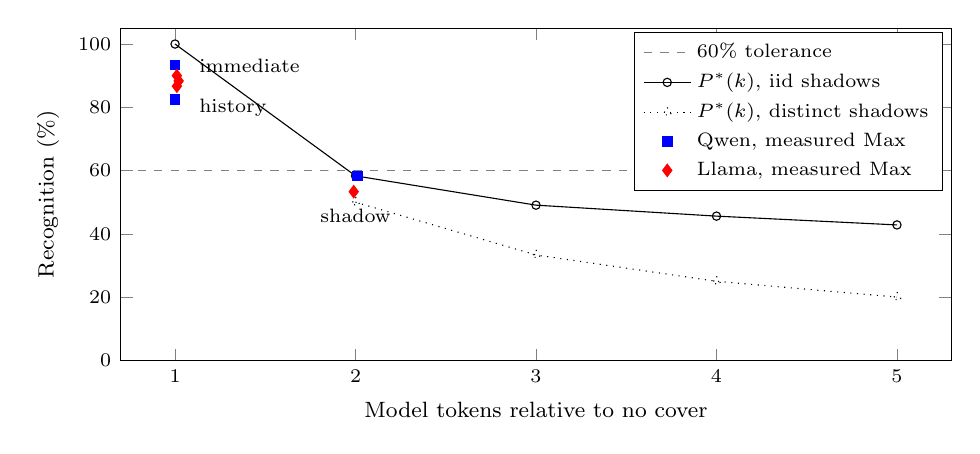
\begin{tikzpicture}
\begin{axis}[width=\columnwidth,height=5.8cm,xmin=0.7,xmax=5.3,ymin=0,ymax=105,
 xlabel={Model tokens relative to no cover},ylabel={Recognition (\%)},
 xtick={1,2,3,4,5},ytick={0,20,40,60,80,100},
 legend style={font=\scriptsize,at={(0.99,0.99)},anchor=north east,cells={anchor=west}},
 tick label style={font=\scriptsize},label style={font=\footnotesize}]
\addplot[gray,dashed,mark=none,domain=0.7:5.3] {60};
\addlegendentry{60\% tolerance}
\addplot[black,mark=o,mark size=1.5pt] coordinates {(1,100) (2,58.33) (3,49.07) (4,45.60) (5,42.82)};
\addlegendentry{$P^*(k)$, iid shadows}
\addplot[black,dotted,mark=triangle,mark size=1.8pt] coordinates {(2,50) (3,33.33) (4,25) (5,20)};
\addlegendentry{$P^*(k)$, distinct shadows}
\addplot[only marks,blue,mark=square*,mark size=1.7pt] coordinates {(1,93.33) (1,82.5) (1,82.5) (2.01,58.33)};
\addlegendentry{Qwen, measured Max}
\addplot[only marks,red,mark=diamond*,mark size=2.2pt] coordinates {(1.01,90) (1.01,86.67) (1.02,88.33) (1.99,53.33)};
\addlegendentry{Llama, measured Max}
\node[font=\scriptsize,anchor=west] at (axis cs:1.08,93) {immediate};
\node[font=\scriptsize,anchor=west] at (axis cs:1.08,80) {history};
\node[font=\scriptsize,anchor=north] at (axis cs:2,51) {shadow};
\end{axis}
\end{tikzpicture}
\caption{Inference--cost frontier against the call-window observer. Points are the strongest tested attacks for the four cover arms; lines are the derived pair-ambiguity floors for $k=0$--4 shadows. Only $k=1$ with iid labels was measured. Controller cover costs no model work but leaves 83--93\% recognition; the measured shadow sits on its floor.}\label{fig:frontier}
\end{figure}


\section{Discussion}\label{sec:discussion}
\paragraph{Design implications}
Four lessons follow for executed cover. First, choose the dispatcher before the cover content: cover that does not pass through a model wait carries a timing signature that removal attacks exploit. Second, matching marginal gaps is insufficient; achieved timing and chronological context remain informative, so a schedule must be evaluated on the records an observer actually sees. Third, planner cover is limited by $P^*(k)$, which falls slowly with more shadows and their linear token cost, whereas drawing shadow labels without replacement lowers it to $1/(k+1)$ at no extra cost; this is the cheapest improvement our analysis predicts and should be measured next. Fourth, isolation is necessary but not sufficient: hidden isolated cover still changes planning paths, and only a state check against declared invariants detects collateral writes.

\paragraph{Threats to validity}\label{sec:limits}
All runs are on one host over loopback, with synthetic tools, two fixed 8B models, and fixtures and phrasings reused across splits and studies. Loopback timing is cleaner than a wide-area path, so the timing attacks may be optimistic for a remote observer; network jitter and loss, cross-host deployment and unseen phrasings are untested. The recipient observer of Table~\ref{tab:cover-necessity}, which also reads decoy arguments, is not measured, and the exact real-chain test for shadow requires per-fixture predictions not reported here. Same-service calls serialize; unknown-task discovery and unrestricted multiplexing are not evaluated. The decision tolerances were set after the measurements. Persistent caches and phase order affect costs. The gap of Section~\ref{sec:gap} concerns four settings from two sources, one of them a preprint; twelve of the fifteen mapped studies are preprints.

\paragraph{Open measurements}
The results call for four measurements: a shadow sweep over $k$ and over iid versus distinct label sampling, with the exact real-chain test; the recipient view, using the per-service request journals; jitter, loss and cross-host deployments with unseen phrasings; and equal-budget comparisons of controller and planner cover under production state contracts with legitimate concurrent updates. Supplement S8 specifies further open questions on feedback attribution and task discovery.

\section{Related Work}\label{sec:related}
\paragraph{Agent side channels}
Section~\ref{sec:background} and Appendix~\ref{app:map} cover attacks on Agent traffic. Closest to our setting, WRA evaluates research decoys and destination visibility against a transit observer~\cite{jeong2026wra}, and the communication-graph study evaluates metadata transformations and live OHTTP~\cite{dangol2026workflow}; neither reports matched task utility for executed cover. Serving-side work shows that token streams, cache sharing and token counts leak through model interfaces~\cite{weiss2024prompt,whisperleak2025,earlybird2025,timewilltell2024,carlini2024timing,wu2026cacheprune}.

\paragraph{Traffic-analysis defenses}
WF defenses pad, pace and add dummy traffic, and their evaluation methodology, including adapted attacks and matched overheads, is well developed~\cite{juarez2014critical,mathews2023critical,dyer2012peekaboo,wang2017walkietalkie,gong2020front,juarez2016wtfpad,shmatikov2006adaptive,cai2014tamaraw}. Smart-home traffic shaping discards cover at a tunnel endpoint~\cite{apthorpe2019stp}. We carry their evaluation obligations over to cover that executes, and add business state and the dispatcher.

\paragraph{Agent security}
Information-flow and privilege controls such as CaMeL, FIDES and Progent restrict what tools an Agent may call and what information flows between them~\cite{debenedetti2025camel,costa2025fides,shi2025progent}; CaMeL explicitly notes tool-call and timing side channels. SPILLage studies behavioral oversharing by browser Agents~\cite{roh2026spillage}. $\tau$-bench and AgentDojo evaluate environment outcomes~\cite{yao2024taubench,debenedetti2024agentdojo}; our state endpoint follows their practice and binds it to traffic measurements. Surveys organize Agent threats by lifecycle and attack surface~\cite{yao2024survey,shahriar2025survey,ferrag2025survey}.

\section{Ethics and Availability}\label{sec:validity}
\paragraph{Ethics}
All experimental inputs are synthetic, and capture filters restrict collection to the experiment. The harmful live-write arm runs on isolated fixtures; no customers or production business states are affected. A hosted retest in Supplement S10 used account-holder authorization; its provider's research terms remain unverified, and it supports no claim in this paper. Traffic inference can enable profiling; our attacks target synthetic tickets only. AI tools assisted extraction, implementation and writing; every measurement is backed by saved observations and executable analysis. Account credentials, hosted-retest captures and transcripts, and third-party full texts are excluded from distribution.

\paragraph{Availability}
All experimental inputs are synthetic, so the artifact can be complete. It contains the collection and analysis code; fixture generators and seeds; frozen plans, validation selections and their hashes; per-episode record metadata, predictions and call truth; the packet captures with their session keys, which belong only to the synthetic test deployment; the forty-four-setting extraction, source locators, blind re-coding sheets and adjudication record; and scripts that rebuild every table. Model weights are public and identified by layer hashes. The artifact is available at \artifacturl.

\section{Conclusion}
When the observer sees the last hop to a third-party tool, privacy cover must execute, and an evaluation must then account for the work it does. We showed that the process dispatching cover determines what leaks: controller cover that skips the model wait is removable, history matching hides that shortcut but not the signal, and a shadow planner is limited by a pair-ambiguity floor that only more model work or label-aware sampling can lower. A goal check alone misses collateral state damage. Binding residual inference, task completion, business state and cost to the same protected executions, and deciding against declared tolerances and a declared observer, turns these measurements into deployment decisions.

\FloatBarrier
\bibliographystyle{IEEEtran}
\bibliography{references}
\appendices
\section{Map of Agent Communication Side-Channel Studies}\label{app:map}
\paragraph{Inclusion and retrieval}
A study is included if an LLM selects actions with external feedback able to affect later actions, and the study links that execution to a communication-side inference or an evaluated protection. Client, tool, model and inter-agent interfaces are eligible; transit, recipient and active observers remain separate. Whole semantic trajectories or browser instrumentation alone, deliberate covert messages and prompt-injection defenses without a communication-side endpoint are excluded~\cite{yao2026intentminer,uitraces2026}. The window covers first public submissions from 1 January 2024 through 9 November 2026. Twelve topic queries, a native arXiv query (180 records) and public-web queries (33 scholarly candidates) gave 209 records after deduplication; two citation leads brought screening to 211, of which fourteen were direct, forty adjacent, 155 outside scope and two unresolved. A retained published seed (CHeaT) gives fifteen direct sources with forty-four settings. Twelve of the fifteen lack a verified formal publication at the cutoff. Exact queries and dispositions are in Supplement S4.

\paragraph{Coding and reliability}
Each setting record binds source version and locator to access, features, learner, target, population, split, intervention, result and cost. We assigned and decided every code against the cited passage; AI tools located candidate passages and proposed drafts, which we accepted, changed or rejected. An independent security PhD researcher, blind to the manuscript and our codes, re-coded the decision-critical subset from the sources without AI tools. Access class (44/44), intervention purpose (9/9), and adaptation and utility in the four privacy settings (4/4 each) agree fully ($\kappa=1$); the protection flag agrees on 38/44 ($\kappa=.61$) and transfer relations on 5/6 ($\kappa=.77$). After adjudication of the seven disagreements against the sources, no privacy setting has both an adapted attacker and matched utility (Supplement S6.1).

\paragraph{The map}
Tables~\ref{tab:complete-matrix-a}--\ref{tab:complete-matrix-b} list all forty-four settings. Twenty-two use transit observations, ten recipient access, eleven active access and one inferred preferences. Three settings compare identity obfuscation and two adversarial-Agent blocking; thirty-four contain no protection comparison. Scores keep their source-defined metric and target and are not cross-paper rankings. Table~\ref{tab:transfer-matrix} relates the Agent evidence to established traffic-analysis conditions: a condition is \emph{retained} when it applies directly, \emph{extended} when an execution condition must be added, \emph{untested} when the Agent evidence does not evaluate it, and an \emph{access mismatch} when host instrumentation is mistaken for passive observation.

\begin{table*}[t]\centering\footnotesize
\caption{Complete setting matrix, part 1 of 2. Each row is one of the forty-four retained settings. Scores keep the source's metric and target; they are not cross-paper rankings. Access states the observer's rights. Last column gives intervention purpose and, for the four privacy comparisons, adapted attack / same-intervention original-task utility (yes or NR: not located). A dash is outside that denominator. Shared* is counted with CG-transform. Full features, split rules and locators remain in the extraction sheet.}\label{tab:complete-matrix-a}
\setlength{\tabcolsep}{3pt}\renewcommand{\arraystretch}{1.12}
\begin{tabularx}{\textwidth}{@{}P{.14\textwidth}P{.11\textwidth}P{.13\textwidth}P{.14\textwidth}P{.12\textwidth}Y P{.09\textwidth}@{}}\toprule
Work / setting & Link; access & Target & Signal / learner & Evaluation unit & Source result & Purpose; A/U \\\midrule

AP-identity~\cite{agentprint2025} & client; transit & hosted-agent identity & Packet size/direction; CNN & interaction & F1 .8660 closed; .8477 open & none; -- \\
AP-behavior~\cite{agentprint2025} & client; transit & interaction mode & Packet size/direction; CNN & interaction & F1 .924/.889 conflict & none; -- \\
AP-persona~\cite{agentprint2025} & preferences; derived & occupation & Inferred preferences & participant preferences & Top-3 occupation 69.1\% & none; -- \\
WRA-prompt~\cite{jeong2026wra} & tool/Web; transit & prompt meaning & Domains/time; LLM & research task & Query recovery .770 / .725 & none; -- \\
WRA-persona~\cite{jeong2026wra} & tool/Web; transit & user traits & Domains/time; LLM & multiple sessions & Separate trait-category scores & none; -- \\
WRA-decoy~\cite{jeong2026wra} & tool/Web; transit & prompt meaning & Domains/time; LLM & research task & .770 to .565; five decoys & privacy; NR/NR \\
WRA-visibility~\cite{jeong2026wra} & tool/Web; transit & prompt meaning & Domains/time; LLM & research task & .770/.610; quality 8.55/8.54 & privacy; NR/yes \\
CG-workflow~\cite{dangol2026workflow} & coord.; transit & workflow class & Graph/size/time; RF & workflow & Nine-class accuracy .67 & none; -- \\
CG-composition~\cite{dangol2026workflow} & coord.; transit & workflow class & Graph/size/time; RF & workflow & Known-label holdout .18 & shared*; -- \\
CG-MCP~\cite{dangol2026workflow} & tool; transit & sequence class & Graph/size/time; RF & fixed sequence & Fixed-sequence accuracy .99 & none; -- \\
CG-transform~\cite{dangol2026workflow} & coord.; transit & workflow class & Graph/size/time; RF & workflow & Capture transformation; separate from live & privacy; yes/NR \\
CG-live~\cite{dangol2026workflow} & coord.; transit & workflow class & Graph/size/time; RF & workflow & Six-class .30; 13x bytes, 11x delay & privacy; yes/NR \\
CG-active~\cite{dangol2026workflow} & coord.; active & integrity impact & Graph/size/time; RF & pending workflow & Live integrity endpoint & none; -- \\
CB-task~\cite{pouryousef2026traffic} & model; transit & task & Traffic statistics; RF & MARBLE execution & Ten-class BA .853/.860 & none; -- \\
CB-topology~\cite{pouryousef2026traffic} & model; transit & task & Traffic statistics; RF & execution & Topology change .83 to .52 & none; -- \\
CB-size-excluded~\cite{pouryousef2026traffic} & model; transit & task class & Traffic statistics; RF & execution & BA .540/.587 & none; -- \\
CB-partial~\cite{pouryousef2026traffic} & model; transit & task & Traffic statistics; RF & execution & One-agent BA .665/.780 & none; -- \\
PF-session~\cite{song2026personafingerprint} & tool/Web; transit & synthetic persona & Signed intervals; CNN & fixed packet window & Per-site persona F1 .78--.91 & none; -- \\
PF-pooled~\cite{song2026personafingerprint} & tool/Web; transit & synthetic persona & Signed intervals; CNN & packet window & Pooled summaries conflict & none; -- \\
PF-open~\cite{song2026personafingerprint} & tool/Web; transit & persona membership & Signed intervals; CNN & window & Open-world misattribution & none; -- \\
MARK-protocol~\cite{kang2026whoseagent} & tool/Web; recipient & agent stack identity & Protocol/headers & trial & TLS/H2 F1 .725; HTTP .799 & none; -- \\
MARK-combined~\cite{kang2026whoseagent} & tool/Web; recipient & agent identity & Protocol/headers & trial & Combined F1 .971 & none; -- \\
\bottomrule\end{tabularx}\end{table*}

\begin{table*}[t]\centering\footnotesize
\caption{Complete setting matrix, part 2 of 2. Each row is one of the forty-four retained settings. Scores keep the source's metric and target; they are not cross-paper rankings. Access states the observer's rights. Last column gives intervention purpose and, for the four privacy comparisons, adapted attack / same-intervention original-task utility (yes or NR: not located). A dash is outside that denominator. Shared* is counted with CG-transform. Full features, split rules and locators remain in the extraction sheet.}\label{tab:complete-matrix-b}
\setlength{\tabcolsep}{3pt}\renewcommand{\arraystretch}{1.12}
\begin{tabularx}{\textwidth}{@{}P{.14\textwidth}P{.11\textwidth}P{.13\textwidth}P{.14\textwidth}P{.12\textwidth}Y P{.09\textwidth}@{}}\toprule
Work / setting & Link; access & Target & Signal / learner & Evaluation unit & Source result & Purpose; A/U \\\midrule

FAY-network~\cite{fayolle2026webagents} & tool/Web; recipient & implementation & Protocol/site features & connection/request & Layer-specific distinguishability & identity; -- \\
FAY-combined~\cite{fayolle2026webagents} & tool/Web; recipient & agent identity & Protocol/site features & visit & Combined fingerprint view & identity; -- \\
FAY-blocking~\cite{fayolle2026webagents} & tool/Web; active & access outcome & Protocol/site features & visit & Access success; not privacy score & blocking; -- \\
AT-choice~\cite{shahriar2026agenttell} & tool/Web; active & cross-origin fact & Challenge choice & two-origin session & 61.1\% loaded choice; cold-adjusted LS & none; -- \\
ANT-scenario~\cite{li2026ant} & egress; transit & scenario & Direction/size/time & episode & Five-task accuracy .431--.727 & none; -- \\
ANT-model-scope~\cite{li2026ant} & model/rest; transit & scenario & Direction/size/time & episode & Eight approximate model-view scores & none; -- \\
ANT-risk~\cite{li2026ant} & egress; transit & benchmark risk label & Direction/size/time & episode & 209 episodes; risk recall .15--.95 & none; -- \\
ANT-stage~\cite{li2026ant} & egress; transit & primitive group & Direction/size/time & primitive segment & 47-group accuracy .355--.462 & none; -- \\
CHT-lure~\cite{ayzenshteyn2025cheat} & asset; active & LLM-based visitor presence & Lure/output/challenge & probe interaction & Presence mechanism; no natural F1 & none; -- \\
CHT-password~\cite{ayzenshteyn2025cheat} & output; active & LLM presence & Lure/output/challenge & challenge response & Password-output control & none; -- \\
CHT-blocking~\cite{ayzenshteyn2025cheat} & CTF; active & defender prevention success & Lure/output/challenge & CTF attempt & CTF prevention endpoint & blocking; -- \\
PT-metadata~\cite{duan2026privacytrace} & tool; recipient & profile attributes & Tool metadata/arguments & single-domain trajectory & ASR .1453; prior .1797 & none; -- \\
PT-content~\cite{duan2026privacytrace} & tool; recipient & profile attributes & Tool metadata/arguments & single-domain trajectory & Arguments ASR .2771 & none; -- \\
ATR-main~\cite{zhao2026agenttrace} & tool; active & model identity & Arguments/repairs & multi-probe attribution trial & 50-probe accuracy .960 & none; -- \\
ATR-budget~\cite{zhao2026agenttrace} & tool; active & model identity & Arguments/repairs & multi-probe attribution trial & 1--50 probes: .652--.960 & none; -- \\
ATR-obfuscation~\cite{zhao2026agenttrace} & tool; active & model identity & Arguments/repairs & multi-probe attribution trial & Attribution above .94 & identity; -- \\
TR-within~\cite{ediga2026trace} & terminal; recipient & model family & Terminal n-grams; SVM & terminal session & Mixed-session F1 .981 & none; -- \\
TR-scaffold~\cite{ediga2026trace} & terminal; recipient & model family & Terminal n-grams; SVM & terminal session & Scaffold holdout F1 .815 & none; -- \\
TR-proprietary~\cite{ediga2026trace} & terminal; recipient & model family & Terminal n-grams; SVM & terminal session & Accuracy .78; narrower models & none; -- \\
HTTP-signature~\cite{borysenko2026http} & docs; recipient & implementation & HTTP trace & documentation-retrieval trial & 9 agents/6 services; descriptive & none; -- \\
HP-calibration~\cite{reworr2024honeypot} & SSH; active & Agent candidate & Timing/prompt responses & controlled probe interaction & Probe timing about 1.7s & none; -- \\
HP-field~\cite{reworr2024honeypot} & SSH; active & Agent candidate & Timing/prompt responses & field interaction/session & 8 candidates; identity unverified & none; -- \\
\bottomrule\end{tabularx}\end{table*}

\begin{table*}[t]\centering\small
\caption{Transfer of established conditions to Agent execution. Relationship labels concern the stated mapping; evidence strength and missing tests appear separately. A missing Agent test does not refute the classical result.}\label{tab:transfer-matrix}
\setlength{\tabcolsep}{4pt}
\begin{tabularx}{\textwidth}{@{}P{.25\textwidth}P{.29\textwidth}P{.10\textwidth}Y@{}}\toprule
Established relation and condition & Agent mapping / consequence & Relation & Agent evidence and remaining test \\\midrule
Unknown boundaries and background affect event recognition~\cite{wang2016realistic,guan2021bapm,deng2023ares,trimananda2020pingpong}. & Tool bursts, model waits and task intervals are different units. Evaluate proposed events with false alarms as well as classification. & Extended & ANT supplies stage boundaries; the concurrent feedback study (Supplement S10) tests particular detectors. Greater Agent localization difficulty is untested. \\\addlinespace[3pt]
Defense evaluation must allow adaptation to the protected distribution~\cite{dyer2012peekaboo,mathews2023critical,tramer2020adaptive}. & Record protected training access and still-visible links; an unchanged learner family can refit. & Retained & Transformed and live OHTTP settings report adaptation in one preprint~\cite{dangol2026workflow}; WRA's matched protected examples remain unresolved. \\\addlinespace[3pt]
Coarse timing/volume can remain useful under specified padding~\cite{dyer2012peekaboo}; serving streams expose length/gap signals~\cite{weiss2024prompt,whisperleak2025}. & Name the shaping policy, receiving hop and Agent workload before carrying over a measured effect. & Untested generalization & Cloud and ANT measure model-view recognition~\cite{pouryousef2026traffic,li2026ant}. A general protected-Agent SSE claim is not tested by these observations. \\\addlinespace[3pt]
An observation result is tied to the visible paths and representations~\cite{chen2010web,apthorpe2019stp}. & Feedback forwards tool information into later model requests across separately controlled services; evaluate every permitted residual view. & Extended & Published WRA tool-side evidence and preprint model/recipient results establish different exposed interfaces. Causal feedback attribution needs its own test. \\\addlinespace[3pt]
STP tunnel endpoints remove cover before it reaches devices or servers~\cite[Sec.~7.1]{apthorpe2019stp}. & When cover executes as research, add original-task resource, state and feedback constraints to the traffic budget. & Extended & Published WRA reports executed research decoys and utility under a different intervention~\cite{jeong2026wra}. Our controlled LLM case separates task completion from state integrity (Section~\ref{sec:state}); it does not evaluate WRA writes. \\\addlinespace[3pt]
Host traces can reconstruct distributed request paths~\cite{reynolds2006wap5,tak2009vpath}. & Instrumentation can provide ground truth; a transit attacker must infer from its own permitted observations. & Access mismatch & ANT stage labels and local task intervals are evaluator-provided. Host tracing alone cannot establish passive encrypted-stream localization. \\\bottomrule
\end{tabularx}
\end{table*}



\section{Defense Design Space}\label{app:defense}
Table~\ref{tab:defense-space} lists defense layers, what each requires the defender to control, the costs to measure together and the exposure that remains.

\begin{table*}[t]\centering\small
\caption{Defense design space: enforcement authority, costs to measure and remaining exposure. Source-specific measurements appear in the text and Supplement S7.}
\label{tab:defense-space}
\setlength{\tabcolsep}{4pt}
\begin{tabularx}{\textwidth}{@{}P{.17\textwidth}P{.25\textwidth}P{.23\textwidth}Y@{}}\toprule
Layer / mechanism & What must be trusted or controlled & Costs to measure together & Residual exposure and practical decision \\\midrule
Naming / association: encrypted name resolution, relays, OHTTP & Name resolver or relay placement; the parties able to link the user to the destination & Added hops, bytes, latency and availability & Shape can survive name hiding. Choose this layer when destination association is the private target; then test remaining observers. \\\addlinespace[3pt]
Representation: message, TLS-record or packet padding & Component that controls the final visible size; padding survives later encoding & Added bytes, record/packet count, fragmentation & Timing, count and other links remain. State the padding layer and test downstream captures. \\\addlinespace[3pt]
Scheduling: batching, pacing, fixed-rate cover & Sender/relay controls output schedule and cover lifetime & First-response delay, completion delay, bandwidth during idle periods & Admission, termination and overflow can reveal activity. Budget these events as part of the visible trace. \\\addlinespace[3pt]
Transport cover: dummy exchanges discarded at a tunnel endpoint & Trusted cover terminator; no dispatch into business tools & Cover bandwidth, queueing, resource use & Other endpoints still see their inputs. Prefer this boundary when the aim is traffic shaping without extra business work. \\\addlinespace[3pt]
Execution cover: extra research or tool calls & Tool privileges, isolated state and whether decoy feedback reaches the planner & Model tokens, tool quota, task success, state changes and latency & A decoy can affect the real execution. Measure privacy and original-task utility on the same protected runs. \\\addlinespace[3pt]
Shared-state isolation / minimization & Tenant separation, cache keys and information passed between services & Lost cache reuse, compute, latency, task accuracy & Isolation removes a sharing channel, not every traffic signal. Minimize tool arguments and feedback according to each recipient's role. \\\bottomrule
\end{tabularx}
\end{table*}


\end{document}
